\documentclass[10pt,a4paper]{report}
\usepackage[utf8x]{inputenc}
\usepackage{graphicx}
\usepackage{ucs}
\usepackage{amsmath}
\usepackage{amsfonts}
\usepackage{amssymb}
\usepackage{makeidx}
\title{Plataforma de Hardware Reconfigurable}
\author{Luis Alberto Guanuco}
\begin{document}
\maketitle
\section*{Intruducción cambiada desde NANO}
A continuación se detallan los avances que se ha logrado de la Pltaforma de Hardware Reconfigurable (PHR).
Se especificará las característica de los componentes seleccionados para luego definir, en diagramas de bloque, el diseño de una placa prototipo que permitirá realizar mediciones y observaciones previas a la placa final.
Se describira el alcance de la Plataforma de Hardware Reconfigurable para luego enumerar los perifericos que se han de implementar en el diseño final.
Finalmente se presenta un esquema posible de la PHR final.
\section*{Esquema de la Plataforma de Hardware Reconfigurable}
Se presenta a continuación un esquema en bloque de su estructura básica.
\begin{figure}
 \centering
  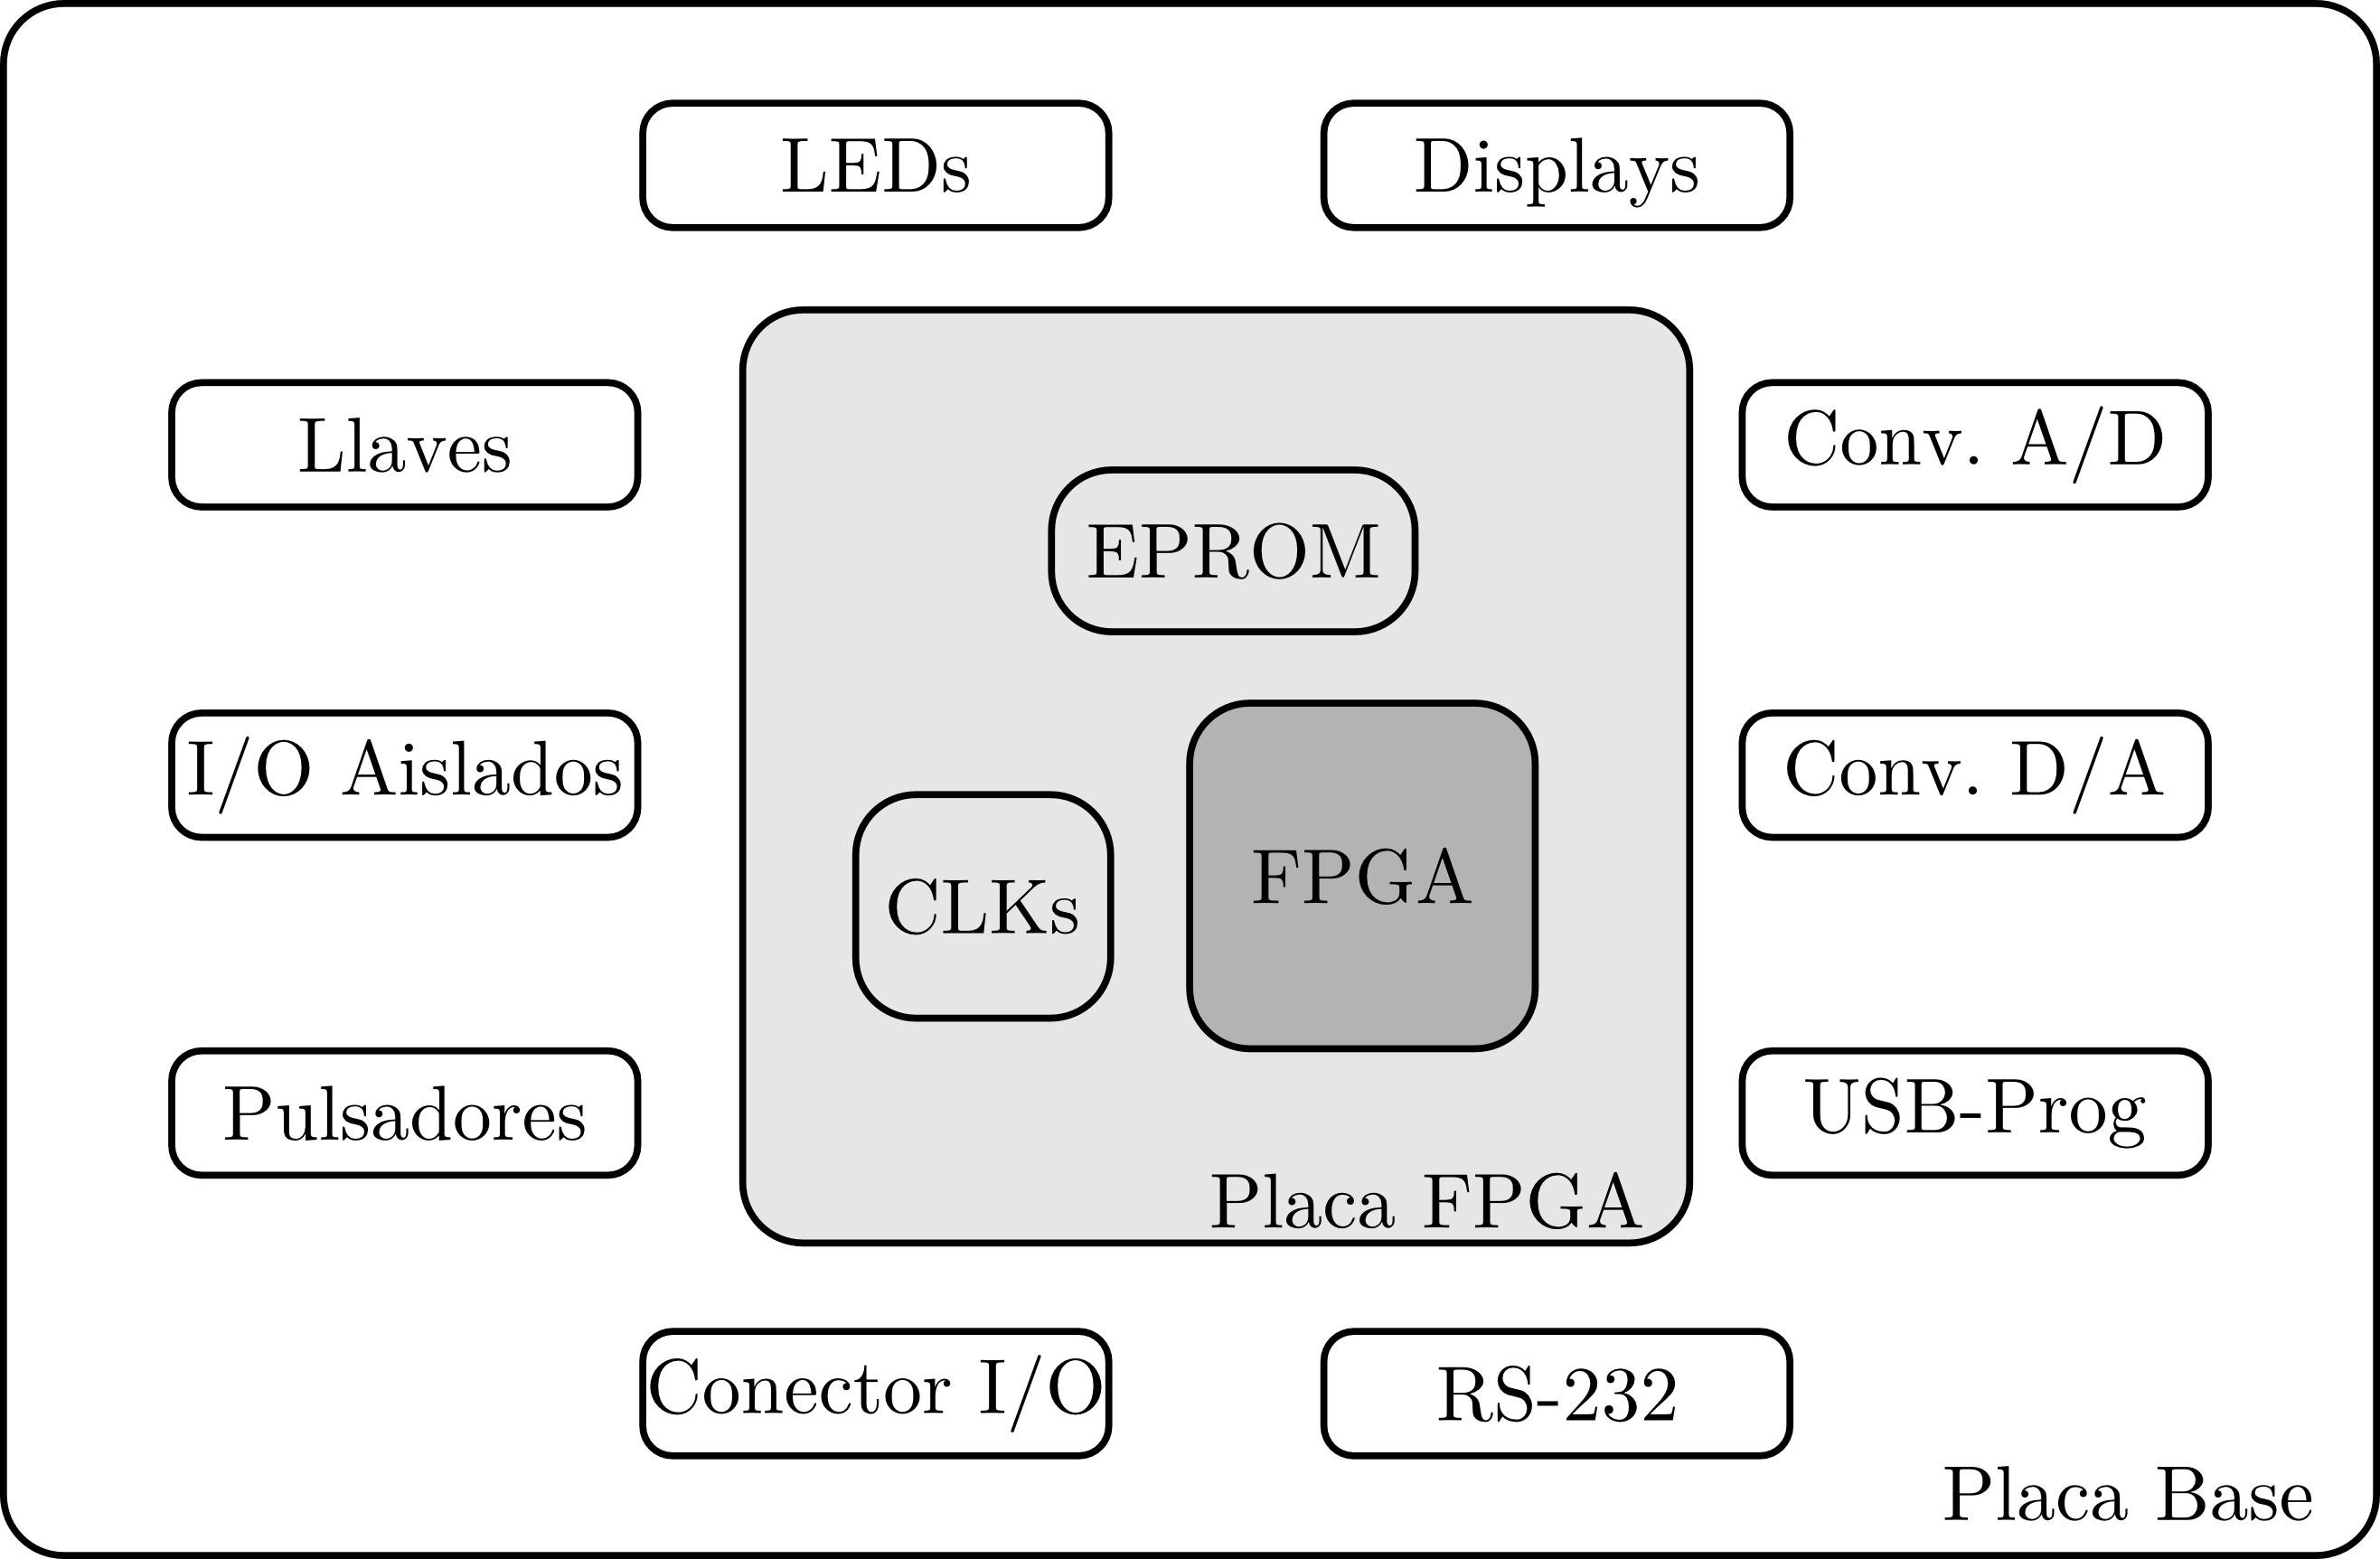
\includegraphics[scale=0.4]{g3018.png}
 \caption{Diagrama en bloque - Plataforma de Hardware Reconfigurable}
\end{figure}
\end{document}
